\documentclass{article}
\usepackage[margin = 0.15in,landscape]{geometry}
\usepackage{multicol}
\usepackage{array}
\usepackage{amsmath}
\usepackage{amssymb}
\usepackage{lmodern}
\usepackage{graphicx}
\usepackage{enumitem}
\setlength\parindent{0pt}
%\renewcommand{\baselinestretch}{0.75}


\begin{document}
\begin{multicols*}{3}
    Marissa Palamara\par 
    ASEN 3112\par 
    Spring 2021
    %\vspace{-0.2cm}
    \setlist{nolistsep}
    % ----- Introduction to Second Law ----- %
    \section*{2nd Law}
    \textbf{The Second Law of Thermodynamics}: Processes occur in a certain direction and energy has quality as well as quantity.\par
    \textbf{Thermal Energy Reservoirs}: A hypothetical body with a relatively large thermal energy capacity (mass x specific heat) that can supply or absorb finite amounts of heat without undergoing any change in temperature. 
    % Heat Engines
    \subsection*{Heat Engines}
    \begin{itemize}
        \item Devices that convert heat to work
        \item Receive heat from high-temp source
        \item Convert part of this heat to work
        \item Reject remaining waste heat to low-temperature sink - Kelvin-Plank Statement
        \item Operate on a cycle
        \item MUST waste some energy by transferring to low-temperature reservoir in order to complete cycle
    \end{itemize}
    Notation:
    \begin{itemize}
        \item $Q_{in}=Q_H$ = amount of heat supplied from a high-temp source
        \item $Q_{out}=Q_L$ = amount of heat rejected to a low temperature sink
        \item $W_{out}$ = amount of work delivered out of system by working fluid
        \item $W_{in}$ = amount of work input to system
    \end{itemize}
    $W_{net,out}=W_{out}-W_{in}\text{ (kJ)}$\par 
    $W_{net,out}=Q_{in}-Q_{out}\text{ (kJ)}$
    % Thermal Efficiency
    \subsection*{Thermal Efficiency}
    $\eta = \frac{W_{net,out}}{Q_{in}}=1-\frac{Q_{out}}{Q_{in}}=1-\frac{Q_L}{Q_H}$
    % Refrigerators and Heat Pumps
    \subsection*{Refrigerators and Heat Pumps}
    \textbf{Coefficient of Performance}: efficiency of a refrigerator.\par 
    $\text{COP}_R=\frac{\text{Desired Output}}{\text{Required Input}}=\frac{Q_L}{W_{net,in}}=\frac{Q_L}{Q_H-Q_L}=\frac{1}{Q_H/Q_L-1}$ \par 
    \textbf{Clausius Statement}: It is impossible to construct a device that operates in a cycle and produces no effect other than the transfer of heat from a lower-temperature body to a higher-temperature body.\par
    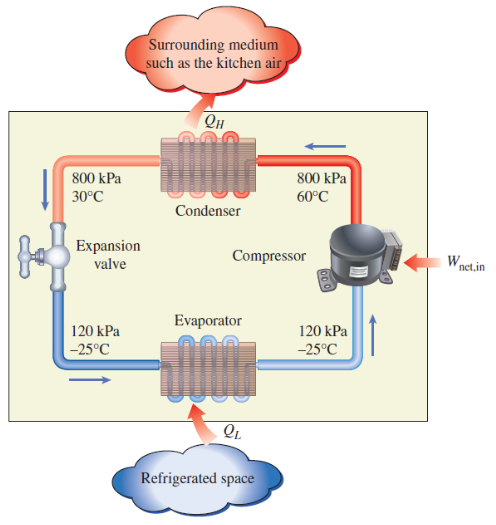
\includegraphics[width=0.75\linewidth]{Images/refrigerator.png}
    \subsection*{Reversible and Irreversible Processes}
    \textbf{Reversible Process}: A process that can be reversed without leaving any trace on the surroundings - theoretical to find limits.\par 
    \textbf{Irreversible Process}: A process that is not reversible.\par 
    \textbf{Ierreversibilities}:
    \begin{itemize}
        \item Friction
        \item Unrestrained expansion
        \item Mixing of two fluids
        \item Heat transfer across a finite temperature difference
        \item Electric resistance
        \item Inelastic deformation of solids
        \item Chemical reactions
    \end{itemize}
    % The Carnot Cycle
    \subsection*{The Carnot Cycle}
    The Carnot Cycle is composed of four reversible processes - two isothermal and two adiabatic - and it can be executed either in a closed or steady-flow system.
    \begin{itemize}
        \item Reversible Isothermal Expansion - \\process 1-2, $T_H$ = constant
        \item Reversible Adiabatic Expansion - \\process 2-3, $T_H\rightarrow T_L$
        \item Reversible Isothermal Compression - \\process 3-4, $T_L$ = constant
        \item Reversible Adiabtic Compression - \\process 4-1, $T_L\rightarrow T_H$
    \end{itemize}
    The Carnot Cycle is completely reversible - in which case it becomes the carnot refrigeration cycle.\par
    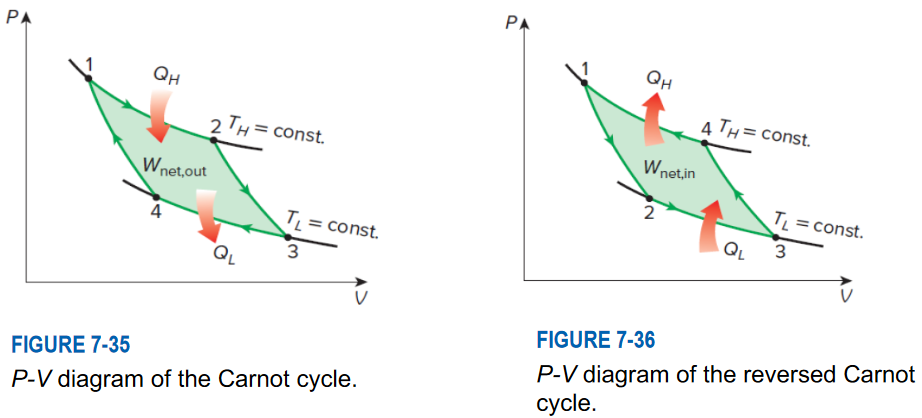
\includegraphics[width=\linewidth]{Images/Pv_Carnot.png}
    \textbf{The Carnot Principles}: The efficiency of an irreversible heat engine is always less than the efficiency of a reversible one operating between the same two reservoirs and the efficiencies of all reversible heat engines operating between the same two reservoirs are the same.\par
    \textbf{The Thermodynamic Temperature Scale}: A temperature scale that is independent of the properties of the substances that are used to measure temperature.\par 
    $T_H=T_L\frac{Q_H}{Q_L}$\par 
    % The Carnot Heat Engine
    \subsection*{The Carnot Heat Engine}
    Any heat engine: $\eta_{th}=1-\frac{Q_L}{Q_H}$\par 
    Carnot heat engine: $\eta_{th,rev}=1-\frac{T_L}{T_H}$\par 
    \begin{equation*}
        \eta_{th}\left\{
            \begin{array}{l}
                <\eta_{th,rev}\text{ irreversible heat engine}\\
                =\eta_{th,rev}\text{ reversible heat engine}\\
                >\eta_{th,rev}\text{ impossible heat engine}
            \end{array}
        \right.
    \end{equation*}
    Amount of heat rejected per cycle: $Q_{L,rev}=\frac{T_L}{T_H}Q_{H,rev}$\par 
    \textbf{Quality of Energy}: The higher the temperature of the thermal energy, the higher its quality. Directly relates to face that you can use temperature to measure efficiency in $\eta_{th,rev}$.
    % The Carnot Refrigerator and Heat Pump
    \subsection*{The Carnot Refrigerator and Heat Pump}
    Any refrigerator or heat pump:\par 
    $\text{COP}_R=\frac{1}{Q_H/Q_L-1}$ and $\text{COP}_{HP}=\frac{1}{1-Q_L/Q_H}$\par 
    Carnot refrigerator or heat pump:\par 
    $\text{COP}_{R,rev}=\frac{1}{T_H/T_L-1}$ and $\text{COP}_{HP,rev}=\frac{1}{1-T_L/T_H}$
    \begin{equation*}
        \text{COP}_{R}\left\{
            \begin{array}{l}
                <\text{COP}_{R,rev}\text{ irreversible refrigerator}\\
                =\text{COP}_{R,rev}\text{ reversible refrigerator}\\
                >\text{COP}_{R,rev}\text{ impossible refrigerator}
            \end{array}
        \right.
    \end{equation*}
    % Begin in lecture 4

\end{multicols*}  
\end{document}